\section{Considerações computacionais para roteirização}\label{sec:considerações computacionais}
Nesta seção, discutem-se questões computacionais de implementação e resolução de problemas de otimização linear e inteira.

\subsection{Metodologia de modelagem em ambiente computacional}
Existem centenas de linguagens de programação, como compilado por \textcite{SCHADE:23}. Excluindo linguagens puramente lúdicas, existe ainda uma vasta gama de linguagens com aplicações práticas que podem ser consideradas para uso neste trabalho, dentre as quais as mais populares são reportadas por \textcite{CARBONNELLE:23}, baseado no número de pesquisas realizadas por tutoriais de programação, fornecido pelo \emph{Google Trends}.

Costumam-se dividir linguagens de programação em duas categorias: de \emph{baixo} e \emph{alto nível}\footnote{\emph{Low-level} e \emph{high-level}, respectivamente.}. Linguagens de baixo nível são aquelas em que "as estruturas de controle e de dados refletem diretamente a arquitetura subjacente da máquina"\footnote{"\textelp{} in which the control and data structures directly reflect the underlying machine architecture."}. Em contrapartida, as linguagens de alto nível são aquelas em que estas estruturas são determinadas pelo problema a ser resolvido \cite{BUTTERFIELD:16}; ou seja, possuem maior nível de abstração.

Em 2000, \textcite{PRECHELT:00} comparou linguagens de programação divididas em três grupos:

\begin{itemize}
    \item Linguagens de alta performance: C e C++, que são de mais baixo nível do que a maioria das linguagens de programação em uso atualmente. Tratam-se de linguagens \emph{compiladas}, o que significa que seu código é transformado em código de máquina\footnote{Em essência, o código que o computador de fato utiliza para executar aplicações \cite{BUTTERFIELD:16}.} para execução. Por esta razão, são utilizadas em projetos que requeiram alta performance e uso eficiente de memória, como sistemas operacionais \cite{TORVALDS:23,WAITE:09};
    \item Linguagem intermediária: Java, separada de C e C++ pela percepção popular de que sua performance é notavelmente inferior à de C e C++ para aplicações pesadas. Java se destaca por sua robustez, tendo se popularizado pelo fato de um mesmo código funcionar em diferentes máquinas \cite{RICARTE:00};
    \item Linguagens de \emph{scripting}: Perl, Python, Rexx e Tcl, que são de mais alto nível. Destas, a que mais se destaca é Python, pela simplicidade de sua sintaxe e o grande número de bibliotecas disponíveis para os mais diversos tipos de aplicação \cite{SRINATH:17}.
\end{itemize}

O autor comparou códigos desenvolvidos por programadores nas diferentes linguagens. O objetivo era resolver um problema que envolvia carregar um grande conjunto de dados na memória e depois retornar uma saída em formato de texto pesquisando pelos dados armazenados. Prechelt concluiu que, em geral, os programas em baixo nível alcançam seus objetivos mais rapidamente. Em contrapartida, os programas em alto nível requerem menos tempo e menos linhas de código para serem implementados. Em termos de produtividade (medida em linhas de código por hora), as linguagens de programação apresentam desempenhos similares. Prechelt reconheceu a simplicidade do problema proposto e admitiu duvidar "\textelp{} que os resultados relativos para as linguagens de \emph{script} seriam tão bons aplicados a outros problemas"\footnote{"\textelp{} that the relative results for the script languages group would hold up well when applied to other problems."}.

Em artigo introduzindo a linguagem de programação Julia, os autores \textcite{JULIA} resumem esta situação:

\begin{displayquote}
    O que o programador dinâmico perde em performance, o programador em C e em Fortran perde em produtividade. Um resultado infeliz [disso] é que as áreas mais desafiadoras da computação numérica tiveram os menores benefícios com o aumento da abstração e da produtividade oferecido por linguagens de alto nível. As consequências têm sido mais sérias do que muitos percebem.\footnote{"As much as the dynamic language programmer misses out on performance, though, the C and Fortran programmer misses out on productivity. An unfortunate outcome is that the most challenging areas of numerical computing have benefited the least from the increased abstraction and productivity offered by higher-level languages. The consequences have been more serious than many realize."}
\end{displayquote}

Portanto, o objetivo da linguagem é aproximar a comunidade científica do objetivo de ter uma linguagem de alto nível e de alta performance. Os resultados apresentados por Julia para o conjunto de problemas de teste apresentado em \cite{JULIA} são comparáveis aos de implementações em C e Fortran, além de mostrarem-se mais consistente do que os das demais linguagens testadas.

Para resolver problemas de otimização em Julia, pode-se utilizar o pacote JuMP \cite{JuMP}, que permite a modelagem de problemas de vários tipos. Seu grande diferencial é que o pacote atua como um intermediário entre o programador e o \emph{solver}, que é a ferramenta utilizada para de fato resolver os problemas. A forma como se adicionam restrições a um problema de otimização, por exemplo, são radicalmente diferentes entre os \emph{solvers} Gurobi \cite{GUROBI:22} e GLPK \cite{GLPK}, de modo que a comparação entre \emph{solvers} se torna um processo muito trabalhoso, mesmo para modelos pequenos. O JuMP resolve este problema com uma forma unificada de modelar problemas, podendo traduzi-los automaticamente de \emph{solver} para \emph{solver}.

\begin{exmp}

Considere o problema de otimização extraído de \cite{FERRIS:07}:
\begin{customopti}|s|
  {max}{}{2x_{1}+3x_{2}}{}{}
  \addConstraint{-4x_{1}+3x_{2}}{\leq12}
  \addConstraint{2x_{1}+x_{2}}{\leq6}
  \addConstraint{x_{1}+x_{2}}{\geq3}
  \addConstraint{5x_{1}+x_{2}}{\geq4}
  \addConstraint{x_{1},x_{2}}{\geq0}.
\end{customopti}

Este problema pode ser modelado em JuMP conforme o \cref{cod:ex362jump}.

\begin{listing}[H]
\centering
\inputminted[mathescape,
               linenos,
               numbersep=5pt,
            %   frame=lines,
            % framesep=2mm
            ]{julia}{códigos/ex362jump.jl}
\caption{Código em Julia do exemplo 3-6-2 usando o \texttt{JuMP.jl}.}
\label[code]{cod:ex362jump}
\end{listing}

A linha \julia{lp = Model(GLPK.Optimizer)} especifica que o \emph{solver} desejado é o GLPK. Se, por exemplo, for desejável alterar o \emph{solver} para o Gurobi, é possível fazê-lo com \julia{set_optimizer(lp, Gurobi.Optimizer)}. A chamada \julia{optimize!(lp)} solicita que o \emph{solver} escolhido resolva o problema. A \cref{cod:output362jump} confirma que a resolução foi bem-sucedida.

\begin{listing}[H]
\centering
\floatname{listing}{Saída}
\inputminted[mathescape,
               linenos,
               numbersep=5pt,
            %   frame=lines,
            % framesep=2mm
            ]{text}{códigos/output362jump.txt}
\caption{Saída do exemplo 3-6-2 usando o \texttt{JuMP.jl}.}
\label[output]{cod:output362jump}
\end{listing}

\end{exmp}

Por todas as razões apresentadas, escolheu-se o Julia para implementar todos os códigos deste trabalho.

\subsection{Técnicas de otimização inteira}
Problemas de otimização inteira são de difícil resolução. É necessário utilizar ferramentas capazes de misturar diversas técnicas para resolvê-los. Tais ferramentas são conhecidas como \emph{solvers}\footnote{Uma tradução literal seria "resolvedor".}.

\subsubsection{Técnicas exatas}
Em geral, os \emph{solvers} tentam resolver problemas de otimização inteira utilizando técnicas exatas de resolução. Estas técnicas são preferíveis por conduzirem o problema à solução ótima de fato. Em contrapartida, sua aplicação costuma tornar a resolução dos problemas mais lenta. O contrário de tais técnicas são as \emph{heurísticas} e \emph{meta-heurísticas}, abordadas adiante.

Geralmente, técnicas exatas envolvem resolver versões relaxadas dos problemas de otimização. Em seguida, verifica-se a factibilidade da resolução relaxada e, se necessário, dividem-se os problemas em problemas menores. Repete-se este processo iterativamente até obter-se uma solução que satisfaça as restrições inteiras e seja ótima.

\textcite{BRADLEY:77,MOHAMED:21} comparam problemas de otimização inteira com suas versões relaxadas. É um erro assumir que a solução inteira ótima para um problema pode ser encontrada arredondando-se ou truncando-se o valor do caso relaxado. Isso se deve a dois motivos: a possibilidade de o valor obtido não ser factível e o fato de a solução inteira poder estar radicalmente distante da linear. Para resolver problemas assim, estes autores introduzem a técnica de \emph{branch-and-bound}, resumida a seguir:

\begin{enumerate}[(a)]
    \item Resolve-se a versão relaxada da formulação inicial do problema, $P_0$. Para-se se nenhuma restrição inteira for violada;
    \item Escolhe-se uma variável $x$ que deveria ser inteira, mas tem valor $x = \alpha \notin \mathbb{Z}$, e criam-se dois novos problemas lineares: $P_1$, com restrição $x \leq \lfloor\alpha\rfloor$, e $P_2$, com restrição $x \geq \lceil\alpha\rceil$;
    \item Resolve-se um dos problemas não resolvidos. Se a solução não for a ótima, repete-se (b). Do contrário, para-se.
\end{enumerate}

O resultado deste procedimento é a criação de uma árvore, em que cada nó é um problema e cada folha é um problema a resolver \cite{GUROBI:22}. A decisão sobre qual folha explorar e a estratégia usada para determinar mais rapidamente uma solução ótima dependem da implementação do \emph{solver} \cite{CLAUSEN:99}.

Uma técnica mais robusta é o \emph{branch-and-cut}. Esta ténica amplia o \emph{branch-and-bound} por meio de \emph{planos de corte}, que são restrições que reduzem o tamanho do poliedro do problema sem excluir soluções inteiras \cite{CARRANO:19}. Quanto maior o número de soluções inteiras em que a restrição for ativa, melhor será o plano de corte. Como o poliedro resultante é menor do que o original, é provável que sejam necessárias menos iterações de \emph{branch-and-bound} para resolver o problema.

Um exemplo de plano de corte é o de Gomory. Suponha que a $i$-ésima restrição linear de um problema com $n$ variáveis de decisão seja $\sum_{j = 1}^{n}a_{ij}x_{j} = b_i$. Então, o seu plano de corte de Gomory será a restrição original menos a restrição com todas as constantes arredondadas para baixo \cite{LEUNG:12,RAVELO:20}:

\begin{equation}
    \sum_{j = 1}^{n}(a_{ij} - \lfloor a_{ij} \rfloor) x_{i} \leq b_i - \lfloor b_i \rfloor.
\end{equation}

Métodos ainda mais robustos podem ser utilizados em busca de soluções exatas. Um exemplo é o \emph{branch-and-price}, que adiciona a técnica de geração de colunas ao \emph{branch-and-bound} e envolve resolver um problema principal e um subproblema, que espera-se que reduza o caminho trilhado para se obter a melhor solução. Este método pode ser combinado com o \emph{branch-and-cut}, formando o que é conhecido como \emph{branch-and-cut-and-price} \cite{CHALAWSKY:22,VIEIRA:13}.

\subsubsection{Técnicas heurísticas}\label{sec:técnicas heurísticas}
Heurísticas são métodos aplicados a problemas específicos que podem gerar atalhos em direção à solução ótima. Estes métodos não têm o rigor matemático de algoritmos e, portanto, não existe a garantia de que sua aplicação será eficiente \cite{BUTTERFIELD:16,VIEIRA:13}.

Um exemplo de heurística para resolução do PCV é apresentado por \textcite{SCHERMER:23}. O procedimento é resumido a seguir.

\begin{enumerate}[(a)]
    \item Dado um PCV assimétrico com grafo $G = (\mcal{V}, \mcal{A})$, em que $\mcal{V}$ é o conjunto de vértices e $\mcal{A}$ é o conjunto de arestas do problema, gerar o seguinte modelo:
        \begin{align}
            \min& \sum_{i,j \in \mcal{V}}{x_{ij}c_{ij}}&&\\
            \text{s.a }& \sum_{j \in \mcal{V}}x_{ij} = 1,&\forall i \in \mcal{V},\ i \neq j,&\\
            &            \sum_{i \in \mcal{V}}x_{ij} = 1,&\forall j \in \mcal{V},\ j \neq i,&\\
            &            x_{ii} = 0,&\forall i \in \mcal{V},&\\
            &            x_{ij} \in \{0, 1\},&\forall i, j \in \mcal{V};
        \end{align}
    \item Solicitar que o \emph{solver} resolva o modelo atual do problema;
    \item Procurar pelo menor ciclo na solução gerada pelo \emph{solver}, com conjunto $S\fast$ de vértices, e parar se $S\fast = \mcal{V}$;
    \item Adicionar a restrição $\sum_{i,j \in S\fast}x_{ij} \leq |S\fast| - 1, \forall S\fast\subsetneq \mcal{V}$ ao modelo. Voltar para (b).
\end{enumerate}

Segundo Schermer, ``prevenir apenas o menor ciclo geralmente é o suficiente para quebrar outros subciclos e mantém o modelo pequeno''.\footnote{"\textelp{} preventing just the shortest cycle is often sufficient for breaking other subtours and will keep the model size smaller."} Duas maneiras são apresentadas para implementar esta heurística:

\begin{itemize}
    \item Iterativa: Espera-se que o \emph{solver} finalize sua resolução do problema para procurar pelo menor subciclo gerado. Então, gera-se um novo modelo e solicita-se que o \emph{solver} o resolva desde o início;
    \item Com \emph{lazy constraints}\footnote{Literalmente, "restrições preguiçosas". Estas restrições recebem este nome por passarem a atuar no problema apenas a partir do momento em que são violadas.}: Inclui-se no modelo uma função de \emph{callback}\footnote{Uma função $f$ é função de \emph{callback} quando é passada como argumento para uma função $F$, que, em algum momento, chama $f$ durante sua execução.} que recebe atualizações de \emph{status} do \emph{solver}. Sempre que o \emph{solver} encontra uma solução inteira ótima para o modelo fornecido, esta função procura pelo menor subciclo e o introduz dinamicamente no modelo.
\end{itemize}

Espera-se que o método de \emph{lazy constraints} seja mais eficiente, pois o \emph{solver} retém as informações obtidas sobre o modelo até o momento. Curiosamente, Schermer observou o contrário no teste que realizou para seu modelo de exemplo, demonstrando a natureza probabilística da aplicação de heurísticas ao problema.

Para PRVs, heurísticas mais robustas são necessárias, pois as violações de restrições não são tão óbvias quanto ciclos não-hamiltonianos. Um exemplo é o problema capacitado, que envolve otimizar o trajeto de uma frota de veículos com capacidade máxima de entregas para cada veículo. Além de procurar por ciclos que não incluem o depósito, \textcite{ACHUTHAN:96} propõem uma heurística que faz três pesquisas em subconjuntos de vértices. A primeira procura por violações a restrições dentro de ciclos envolvendo o depósito, a segunda procura por violações fora de cada ciclo e a terceira faz uma checagem final de todos os ciclos para os quais não foram encontradas restrições.

% \begin{align}
%     \text{min\ } &\sum_{i > j}c_{ij}x_{ij}&&\\
%     \text{s.a\ } &\sum_{i \in \mcal{V}\fast}x_{nj} = 2V,&&\\
%     &\sum_{i>k}x_{ik} + \sum_{k>i}x_{ki} = 2,&\forall k \in \mcal{V}\fast,&\\
%     &\sum_{\substack{i,j \in S\\i>j}x_{ij}} \leq |S| - \ell(S),&\forall S \subseteq\mcal{V}\fast, 3 \leq |S| \leq n - 2,&\\
%     &x_{ij} = \begin{cases}
%         \text{0, 1 ou 2 para i = n},\\
%         \text{0 ou 1, do contrário},
%     \end{cases}&&\\
%     &V > 0.&&
% \end{align}

% Nesta formulação, a matriz de adjacência é triangular inferior, sendo utilizados apenas os elementos $x_{ij}$ com $i > j$.

Existem técnicas mais gerais, conhecidas como meta-heurísticas, que podem ser aplicadas a diferentes tipos de problemas e conseguem evitar alguns dos obstáculos enfrentados pelas heurísticas. Exemplos populares já utilizados para resolver PRVs incluem a busca tabu, a colônia de formigas e os algoritmos evolucionários \cite{VIEIRA:13}.

\subsection{Comparações computacionais}
Nesta seção, apresenta-se um método para comparar \emph{solvers} e formulações de roteirização.

\subsubsection{Comparação de formulações}
O objetivo desta seção é demonstrar uma possível comparação de formulações de problemas. Toma-se como base o PCV, devido à maior simplicidade de implementação. No entanto, esta comparação também pode ser feita para diferentes formulações de VRPs.

Em 2021, \textcite{BAZRAFSHAN:21} compararam as três formulações de PCV apresentadas na \cref{sec:PCV}. Os autores analisaram os desempenhos das formulações para 10 problemas diferentes, de 10 a 500 pontos, com coordenadas aleatórias para os vértices. Das três formulações, os autores constataram que a GG é a melhor, seguida pela MTZ. A partir de 19 pontos, a formulação DFJ sequer consegue resolver problemas no tempo limite.

A família de restrições da DFJ é imposta sobre todos os subconjuntos próprios do problema, exceto pelo conjunto vazio. Isso significa que o número de restrições desta família é $|2^\mcal{V}| - 2$, sendo $2^\mcal{V}$ o conjunto potência do conjunto de vértices do problema, $\mcal{V}$. Este crescimento exponencial sobrecarrega o \emph{solver} logo no início da resolução do problema, inviabilizando-a.

Para resolver os problemas relaxados, a formulação MTZ leva vantagem sobre a GG, por adicionar menos variáveis e restrições ao problema. Ainda assim, os autores consideram a GG melhor, pois suas variáveis de ordenação são reais, ao passo que as da MTZ são inteiras. Como resultado, a MTZ tem desempenho inferior quando o modelo é passado da forma relaxada para a forma inteira.

Em relação às formulações do PCV, esta seção tem dois objetivos: verificar se as conclusões de \textcite{BAZRAFSHAN:21} sobre as formulações GG e MTZ se confirmam e comparar estas formulações à DFJ com a técnica de \emph{lazy constraints} apresentada na \cref{sec:técnicas heurísticas}. Para tal, foram criados 3 conjuntos com 10 problemas gerados aleatoriamente em cada um. Os problemas do conjunto A têm 10 pontos; do B, têm 15; e do C têm 20. Em seguida, os problemas foram resolvidos por três \emph{solvers}: GLPK \cite{GLPK}, CPLEX \cite{CPLEX} e Gurobi \cite{GUROBI:22}. Para estes testes, foi utilizado um \emph{IdeaPad} com processador Intel Core i5-10210U, 1.60 GHz, memória de 8 GB e suporte a até 8 \emph{threads}. Os tempos de resolução foram fornecidos pelos próprios \emph{solvers}, gerando a \cref{tab:tempos pcv}. As implementações são fornecidas no \cref{sec:PCV implementações}.

\begin{table}
\centering
\caption{Tempos (s) de resolução para diferentes \emph{solvers} e formulações.}\label{tab:tempos pcv}
\begin{threeparttable}
\begin{tabular}{lccccccccc}
\toprule
& \multicolumn{3}{c}{GLPK} & \multicolumn{3}{c}{CPLEX} & \multicolumn{3}{c}{Gurobi}
\\\cmidrule(lr){2-4}\cmidrule(lr){5-7}\cmidrule(lr){8-10}
           & DFJ* & MTZ & GG & DFJ* & MTZ & GG & DFJ* & MTZ & GG\\\midrule
A1 & $2.964$ & $0.746$ & $\mathbf{0.055}$ & $0.703$ & $0.461$ & $\mathbf{0.046}$ & $0.641$ & $0.333$ & $\mathbf{0.022}$\\
A2 & $\mathbf{0.002}$ & $0.228$ & $0.056$ & $\mathbf{0.008}$ & $0.118$ & $0.050$ & $\mathbf{0.008}$ & $0.191$ & $0.021$\\
A3 & $\mathbf{0.003}$ & $0.087$ & $0.036$ & $\mathbf{0.011}$ & $0.077$ & $0.066$ & $\mathbf{0.006}$ & $0.116$ & $0.016$\\
A4 & $\mathbf{0.002}$ & $0.016$ & $0.035$ & $\mathbf{0.005}$ & $0.026$ & $0.025$ & $\mathbf{0.003}$ & $0.060$ & $0.035$\\
A5 & $\mathbf{0.002}$ & $0.220$ & $0.217$ & $\mathbf{0.005}$ & $0.093$ & $0.039$ & $\mathbf{0.008}$ & $0.149$ & $0.017$\\
A6 & $\mathbf{0.002}$ & $0.032$ & $0.017$ & $\mathbf{0.008}$ & $0.031$ & $0.015$ & $\mathbf{0.006}$ & $0.043$ & $0.015$\\
A7 & $\mathbf{0.007}$ & -- & $0.057$ & $\mathbf{0.012}$ & $0.078$ & $0.044$ & $\mathbf{0.008}$ & $0.085$ & $0.035$\\
A8 & $\mathbf{0.002}$ & $1.188$ & $0.177$ & $\mathbf{0.005}$ & $1.356$ & $0.140$ & $\mathbf{0.004}$ & $0.488$ & $0.059$\\
A9 & $\mathbf{0.004}$ & $0.074$ & $0.089$ & $\mathbf{0.007}$ & $0.031$ & $0.036$ & $\mathbf{0.009}$ & $0.091$ & $0.021$\\
A10 & $\mathbf{0.003}$ & $0.210$ & $0.112$ & $\mathbf{0.013}$ & $0.049$ & $0.057$ & $\mathbf{0.007}$ & $0.178$ & $0.031$\\
B1 & $\mathbf{0.048}$ & $3.341$ & -- & $\mathbf{0.035}$ & $0.354$ & $0.514$ & $\mathbf{0.038}$ & $0.274$ & $0.208$\\
B2 & $\mathbf{0.015}$ & $1.412$ & $1.047$ & $\mathbf{0.061}$ & $0.139$ & $0.377$ & $\mathbf{0.044}$ & $0.371$ & $0.159$\\
B3 & $\mathbf{0.053}$ & -- & $18.238$ & $\mathbf{0.035}$ & $0.215$ & $0.183$ & $\mathbf{0.025}$ & $0.225$ & $0.078$\\
B4 & $\mathbf{0.028}$ & $47.536$ & $0.861$ & $\mathbf{0.037}$ & $18.583$ & $0.218$ & $\mathbf{0.019}$ & $3.612$ & $0.091$\\
B5 & $\mathbf{0.022}$ & $1.244$ & $0.462$ & $\mathbf{0.018}$ & $0.338$ & $0.114$ & $\mathbf{0.019}$ & $0.293$ & $0.063$\\
B6 & $\mathbf{0.006}$ & $0.274$ & $3.103$ & $\mathbf{0.036}$ & $0.074$ & $0.098$ & $\mathbf{0.026}$ & $0.140$ & $0.069$\\
B7 & $\mathbf{0.008}$ & -- & $3.711$ & $\mathbf{0.028}$ & $0.332$ & $0.138$ & $\mathbf{0.012}$ & $0.261$ & $0.134$\\
B8 & $\mathbf{0.022}$ & $2.148$ & $3.205$ & $\mathbf{0.016}$ & $0.540$ & $0.276$ & $\mathbf{0.012}$ & $0.364$ & $0.107$\\
B9 & $\mathbf{0.010}$ & -- & $18.597$ & $\mathbf{0.016}$ & $0.091$ & $0.087$ & $\mathbf{0.011}$ & $0.119$ & $0.063$\\
B10 & $\mathbf{0.019}$ & -- & $43.736$ & $\mathbf{0.036}$ & $18.869$ & $0.192$ & $\mathbf{0.019}$ & $2.609$ & $0.094$\\
C1 & $\mathbf{0.022}$ & -- & -- & $\mathbf{0.061}$ & $2.832$ & $0.127$ & $\mathbf{0.055}$ & $1.485$ & $0.304$\\
C2 & $\mathbf{0.064}$ & $9.668$ & $8.949$ & $\mathbf{0.149}$ & $0.408$ & $0.372$ & $\mathbf{0.046}$ & $1.434$ & $0.135$\\
C3 & $\mathbf{0.012}$ & $11.405$ & -- & $\mathbf{0.026}$ & $0.484$ & $0.501$ & $\mathbf{0.026}$ & $0.372$ & $0.150$\\
C4 & $\mathbf{0.226}$ & -- & -- & $\mathbf{0.116}$ & $8.615$ & $0.428$ & $\mathbf{0.054}$ & $2.957$ & $0.229$\\
C5 & $\mathbf{0.035}$ & $27.043$ & $22.634$ & $\mathbf{0.040}$ & $8.298$ & $0.138$ & $\mathbf{0.021}$ & $3.103$ & $0.241$\\
C6 & $\mathbf{0.023}$ & -- & -- & $\mathbf{0.085}$ & $0.732$ & $1.192$ & $\mathbf{0.059}$ & $1.670$ & $0.234$\\
C7 & $\mathbf{0.160}$ & $13.547$ & -- & $\mathbf{0.049}$ & $1.304$ & $0.531$ & $\mathbf{0.046}$ & $0.918$ & $0.271$\\
C8 & $\mathbf{0.089}$ & -- & $18.351$ & $\mathbf{0.137}$ & $7.881$ & $0.468$ & $\mathbf{0.056}$ & $4.076$ & $0.289$\\
C9 & $\mathbf{0.138}$ & $31.818$ & -- & $\mathbf{0.075}$ & $4.832$ & $0.225$ & $\mathbf{0.052}$ & $2.992$ & $0.130$\\
C10 & $\mathbf{0.074}$ & $1.840$ & -- & $\mathbf{0.057}$ & $0.117$ & $0.271$ & $\mathbf{0.024}$ & $0.244$ & $0.110$\\
\bottomrule
\end{tabular}
\begin{tablenotes}
\item A, conjuntos de 10 pontos; B, conjuntos de 15 pontos; C, conjuntos de 20 pontos; DFJ*, DFJ com \emph{lazy constraints}. Tempos maiores do que 60 s foram desconsiderados e substituídos por travessão.
\end{tablenotes}
\end{threeparttable}
\end{table}

Constata-se que a formulação GG de fato é superior à MTZ para a resolução completa do PCV. Ademais, a formulação DFJ com \emph{lazy constraints} consegue chegar à resposta ótima mais rapidamente do que as demais em todos os testes exceto um. Talvez esta anomalia possa ser explicada por se tratar do primeiro teste realizado com cada \emph{solver}. É possível que os \emph{solvers} contabilizem algum tempo de inicialização adicional nesta situação.

\subsubsection{Comparação de solvers}
Para comparar os \emph{solvers}, utilizou-se a metodologia de Dolan e Moré \cite{DOLAN:02}. Sejam $\mathcal{P}$ e $\mathcal{S}$ conjuntos de problemas e \emph{solvers}, respectivamente. Para todo problema $p \in \mathcal{P}$ e \emph{solver} $s \in \mathcal{S}$, obtém-se uma performance $t_{p,s}$ de acordo com alguma métrica de desempenho (tempo de resolução, número de funções utilizadas, etc.). Então, obtêm-se as razões entre os desempenhos de cada \emph{solver} e o desempenho do melhor \emph{solver} para determinado problema:

\begin{equation}
    r_{p,s} = \frac{t_{p,s}}{\min\{t_{p,s} \mid s \in \mathcal{S}\}}.
\end{equation}

Então, define-se uma função estatística chamada de \emph{performance profile}\footnote{"Perfil de performance."}, que representa uma distribuição das probabilidades de um problema $p \in \mcal{P}$ ser resolvido por um \emph{solver} $s \in \mcal{S}$ dentro de um intervalo $[1,\tau]$ de razões em relação ao resultado do melhor \emph{solver} para o problema em questão:

\begin{equation}
    \rho_s(\tau) = \frac{1}{|\mathcal{P}|}|\{p \in \mathcal{P}\ \mid r_{p,s} \leq \tau\}|.
\end{equation}

Aplicando este procedimento aos resultados da \cref{tab:tempos pcv}, obtêm-se as \cref{fig:pgraph10,fig:pgraph15,fig:pgraph20}, onde são comparados os \emph{performance profiles} dos três \emph{solvers} testados, tomando o DFJ com \emph{lazy constraints} como base.

\begin{figure}
    \centering
    \caption{\emph{Performance profiles} para o conjunto de 10 pontos}
    \label{fig:pgraph10}
    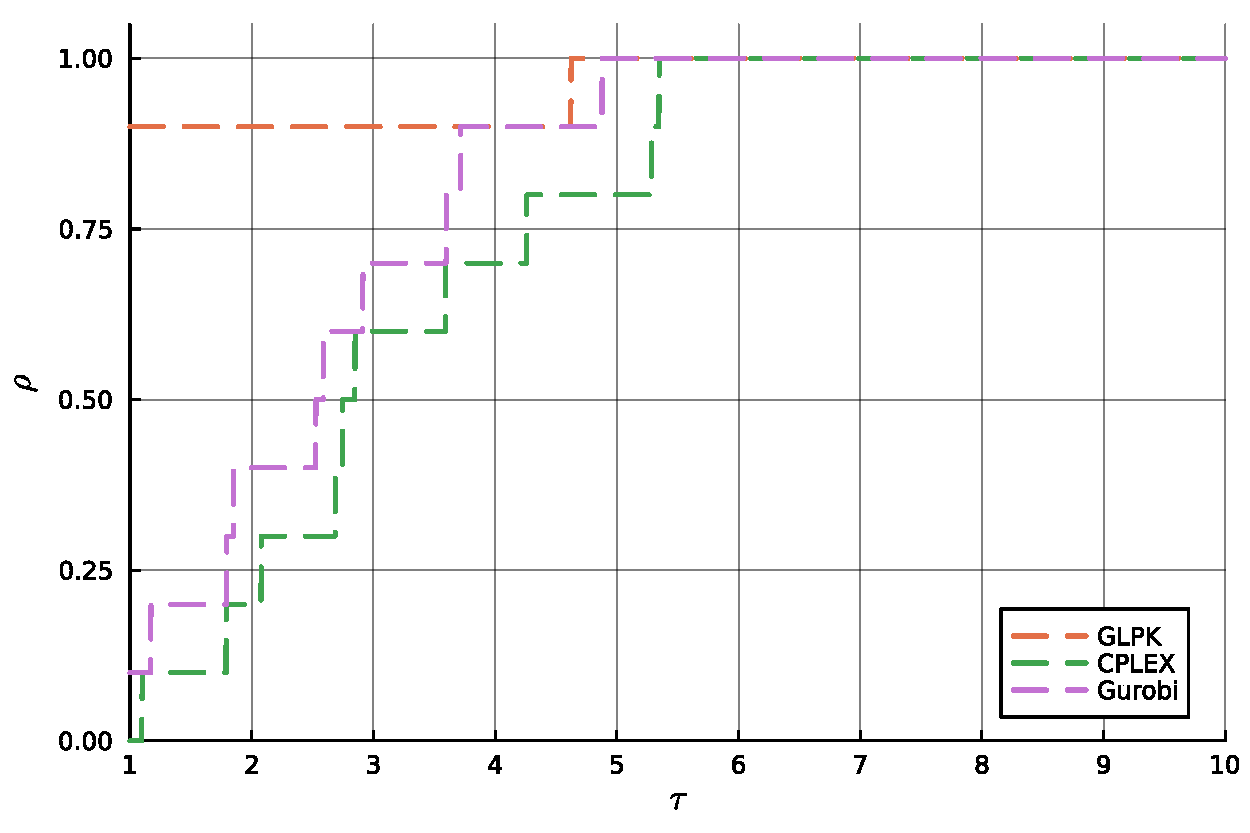
\includegraphics[scale=0.6]{imagens/pgraph10.pdf}
\end{figure}
\begin{figure}
    \centering
    \caption{\emph{Performance profiles} para o conjunto de 15 pontos}
    \label{fig:pgraph15}
    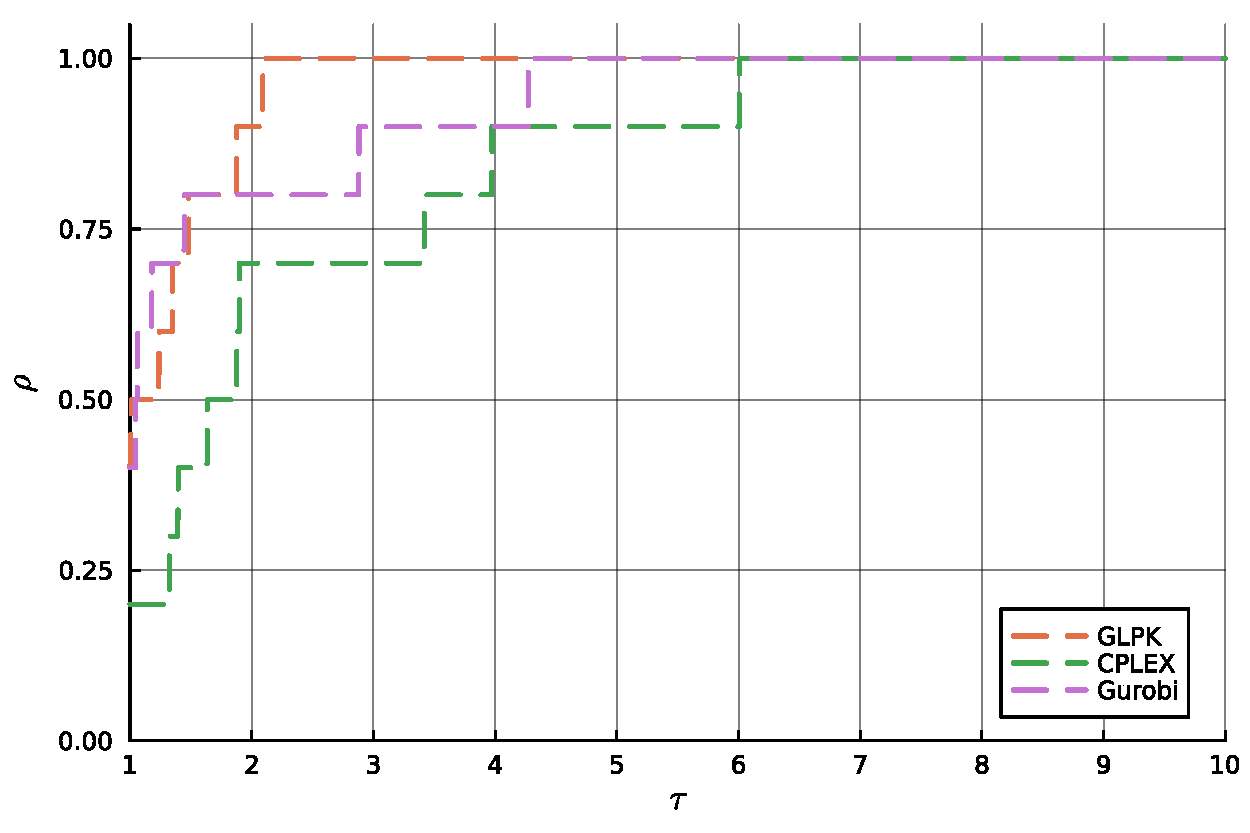
\includegraphics[scale=0.6]{imagens/pgraph15.pdf}
\end{figure}
\begin{figure}
    \centering
    \caption{\emph{Performance profiles} para o conjunto de 20 pontos}
    \label{fig:pgraph20}
    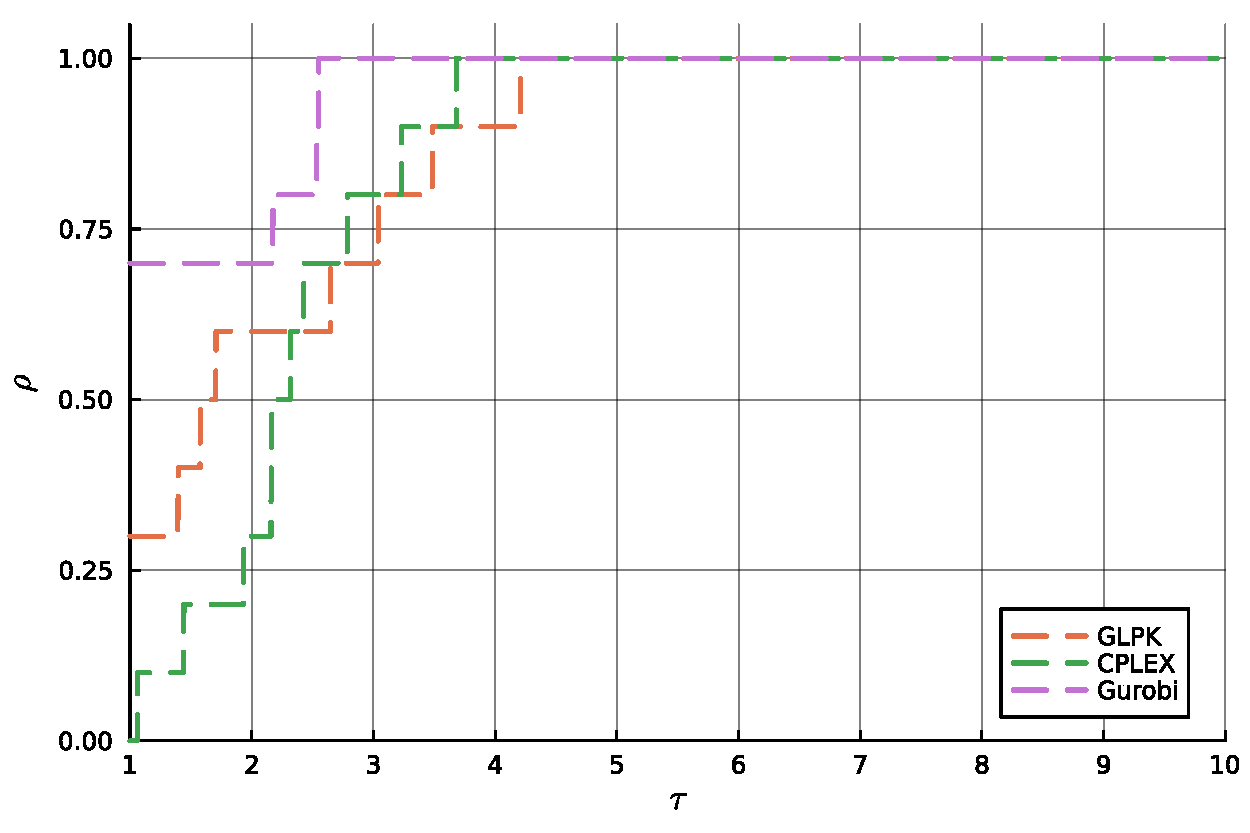
\includegraphics[scale=0.6]{imagens/pgraph20.pdf}
\end{figure}

Cada "degrau" num gráfico de \emph{performance profiles} indica a razão de problemas resolvidos no tempo relativo indicado pelas abscissas. Assim, o \emph{solver} cujo \emph{performance profile} intercepta as ordenadas com valor mais alto é o que chega à solução ótima mais rapidamente na maioria dos casos. Para 10 pontos, o GLPK é dominante neste aspecto. O Gurobi passa a dominar conforme o número de pontos aumenta.

Com 20 pontos, o Gurobi começa a se distanciar dos demais \emph{solvers}. O GLPK e o CPLEX apresentam desempenhos similares. Realizou-se mais um teste, este com 10 problemas de 50 pontos, para verificar a tendência de desempenho dos \emph{solvers} em situações mais extremas. Os resultados são apresentados na \cref{tab:tempos pcv50}.

\begin{table}
\centering
\caption{Tempos (s) de resolução para PCVs de 50 pontos usando DFJ com \emph{lazy constraints}}\label{tab:tempos pcv50}
\begin{threeparttable}
\begin{tabular}{lccc}
\toprule
GLPK & CPLEX & Gurobi\\\midrule
-- & $1.530$ & $\mathbf{0.983}$\\
$13.778$ & $\mathbf{0.312}$ & $0.395$\\
-- & $0.652$ & $\mathbf{0.535}$\\
-- & $\mathbf{0.365}$ & $0.451$\\
-- & $0.598$ & $\mathbf{0.517}$\\
-- & $0.918$ & $\mathbf{0.440}$\\
-- & $0.511$ & $\mathbf{0.381}$\\
-- & $1.523$ & $\mathbf{0.702}$\\
-- & $1.071$ & $\mathbf{0.630}$\\
$35.082$ & $0.747$ & $\mathbf{0.410}$\\
\bottomrule
\end{tabular}
\begin{tablenotes}
\item Tempos maiores do que 60 s foram substituídos por travessão.
\end{tablenotes}
\end{threeparttable}
\end{table}

A \cref{fig:pgraph50} mostra uma comparação dos \emph{performance profiles} para 50 pontos, desconsiderando o GLPK. Verifica-se que o Gurobi continua à frente, apesar de o CPLEX conseguir uma performance comparável, sendo pouco mais que duas vezes mais lento no pior dos casos.

\begin{figure}
    \centering
    \caption{\emph{Performance profiles} para o conjunto de 50 pontos}\label{fig:pgraph50}
    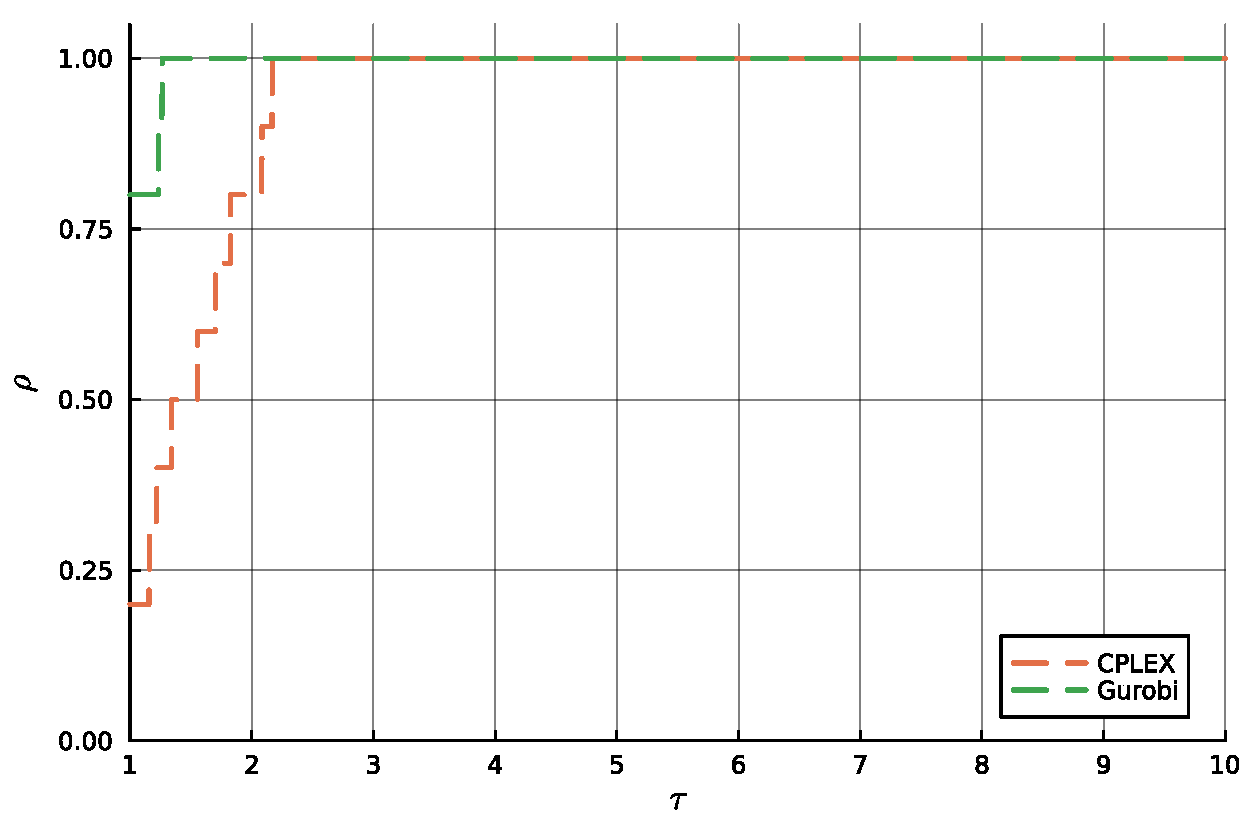
\includegraphics[scale=0.6]{imagens/pgraph50.pdf}
\end{figure}

% \subsection{Problemas de roteamento de veículos}\label{sec:problemas de roteamento de veículos}

% Problemas de roteamento de veículos (PRVs) são extensões do PCV onde mais do que um veículo passa a ser considerado \cite{OR-Tools-VRP}. Geralmente, estes problemas também acrescentam restrições para representar situações mais realistas no roteamento. De particular interesse aqui são o problema de roteamento de veículos capacitado (PRVC) e o problema de roteamento de veículos com janela de tempo (PRVJT).

% O PRVC considera uma frota de veículos com capacidade máxima. Os veículos devem deixar o depósito e realizar entregas de modo que seja necessário apenas um veículo para abastecer cada ponto; ou seja, a capacidade dos veículos deve ser respeitada. O PRVJT, por sua vez, é uma extensão do PRVC, considerando que cada ponto deve ser atendido dentro de determinado intervalo de tempo.

% Existem várias maneiras de formular o PRVJT. Nesta seção, utilizaremos a mostrada por Vieira \cite{VIEIRA:13}, com uma notação um pouco diferente. Considere $\mcal{V}$ o conjunto de vértices do problema, $K$ o conjunto de veículos utilizados, $C$ a capacidade máxima dos veículos, $m_i$ as demandas respectivas dos vértices $v_i$ e $v(S)$ o número de veículos necessários para atender completamente a demanda de um conjunto de vértices $S$.

% Com as variáveis descritas até aqui, temos o suficiente para representar um PRVC. Para representar um PRVJT, entram em jogo as variáveis $b_i$, que indicam o momento de chegada de um veículo a cada vértice $v_i$; $s_i$, que indicam o tempo necessário para atender cada vértice $v_i$; e $t_{ij}$, que indicam o tempo de deslocamento dos vértice $v_i$ para os vértices $v_j$. Por fim, as variáveis $b_i$ e $l_i$ indicam, respectivamente, o começo e o fim do intervalo de tempo em que os vértices estão disponíveis para atendimento.

% Denotando $\mcal{V}\fast = \mcal{V}\backslash\{0\}$, temos o seguinte modelo de PRVJT:

% \begin{subequations}
% \begin{align}
%     \min&\sum_{\substack{i\in \mcal{V} \\ j\in \mcal{V} \\ k\in K}}\vcc{ij}\x{ijk} \label[expression]{eq:prvjt1}\\
%     \text{s.a }&\sum_{\substack{k \in \mcal{V} \\ j \in \mcal{V}\fast}} \x{0jk} \leq |K|,& \label[constraint]{eq:prvjt2}\\
%     &\sum_{j\in \mcal{V}\fast}\x{0jk} = \sum_{j\in \mcal{V}\fast}\x{j0k} \leq 1,&\forall k \in K,& \label[constraint]{eq:prvjt3}\\
%     &\sum_{\substack{k\in K \\ j\in \mcal{V}}}\x{ijk} = 1,&\forall i \in \mcal{V}\fast,& \label[constraint]{eq:prvjt4}\\
%     &\sum_{j\in \mcal{V}}\x{ijk} = \sum_{j \in \mcal{V}}\x{jik},&\forall k \in K,\ i \in \mcal{V}\fast,& \label[constraint]{eq:prvjt5}\\
%     &\sum_{\substack{i\in S \\ j\in S \\ k \in K}}\x{ijk} \leq |S| - v(S),&\forall S \subseteq \mcal{V}\fast,\ |S| \geq 2,& \label[constraint]{eq:prvjt6}\\
%     &\sum_{\substack{i\in \mcal{V}\fast\\j\in \mcal{V} \\ j \neq i}}m_i\x{ijk} \leq C,&\forall k \in K,& \label[constraint]{eq:prvjt7}\\
%     &\sum_{\substack{k \in K \\ i \in \mcal{V} \\ i \neq j}}\x{ijk}(b_i + s_i + t_{ij}) \leq b_j,&\forall j \in \mcal{V}\fast,& \label[constraint]{eq:prvjt8}\\
%     &e_i \leq b_i \leq l_i,&\forall i \in \mcal{V},& \label[constraint]{eq:prvjt9}\\
%     &\x{ijk} \in \{0,1\},&\forall i, j \in \mcal{V},\ k \in K \label[constraint]{eq:prvjt10}.
% \end{align}
% \end{subequations}

% A \cref{eq:prvjt1} generaliza o problema de minimização para vários veículos, enquanto a \cref{eq:prvjt2} garante que o número de veículos utilizados não exceda o total da frota. As \cref{eq:prvjt3,eq:prvjt4,eq:prvjt5} asseguram que todas as rotas terão início e fim no depósito; que de cada ponto (salvo o depósito) ocorre a partida de apenas um veículo; e que um veículo que entre em um ponto deve também sair deste ponto.

% A \cref{eq:prvjt6} é uma versão ampliada da restrição anti-subciclo introduzida na modelagem do PCV, na \cref{sec:pcv}. Note que o número máximo aceitável de deslocamentos dentro de um subconjunto de pontos do problema foi alterado de ${|S| - 1}$ para ${|S| - v(S)}$. Para entender esta alteração, imagine que ${v(S) \geq 1}$ veículos precisem atender um subconjunto de $|S|$ pontos. Como cada veículo inicia sua trajetória neste conjunto a partir de um dos seus pontos, restam $|S| - v(S)$ pontos pelos quais estes veículos podem passar sem voltar a um ponto que já foi atendido anteriormente. Portanto, ${|S| - v(S)}$ é o número máximo de deslocamentos que pode acontecer sem que ocorra formação de subciclos no subconjunto de pontos $S$. Por fim, note que a modelagem de Vieira inclui ainda a condição $S \subseteq \mcal{V}\fast$ nesta restrição, pois a \cref{eq:prvjt3} força todos os veículos que partirem do depósito a retornar para ele, o que torna sua inclusão redundante.

% A \cref{eq:prvjt7} garante que nenhum veículo tenha que entregar mais carga do que consegue comportar. Segundo Vieira, esta restrição é redundante, pois a \cref{eq:prvjt6} implicitamente garante os mesmos resultados.

% A \cref{eq:prvjt8} assegura que os veículos cheguem em horários adequados aos pontos que devem atender. Assim, é necessário que a soma do tempo de chegada ao ponto $i$, do tempo de atendimento ao ponto $i$ e do tempo de deslocamento do ponto $i$ ao $j$ resulte em um tempo igual ou anterior ao momento em que se espera começar a atender o ponto $j$. Este tempo é delimitado pela \cref{eq:prvjt9}, devendo estar dentro do intervalo de disponibilidade do ponto ao qual se chega. Note que a \cref{eq:prvjt8} força os veículos a se deslocarem por entre pontos diferentes, o que impede a formação de subciclos de um único ponto. É por esta razão que a \cref{eq:prvjt6} impõe a condição $\ |S| \geq 2$.

% Existem várias outras considerações a fazer, a depender do caso. Por exemplo, Kallehauge \emph{et al.} \cite{KALLEHAUGE:05} apresentam a possibilidade de se modelar o problema considerando que diferentes veículos podem levar diferentes tempos para atender a certos pontos. Isso introduz não-linearidades ao modelo, deixando sua resolução mais complexa. No fim das contas, é necessário avaliar quão realista e precisa a modelagem de um problema tem que ser para optar por um modelo ou outro.